\section{Overview}
\label{sec:overview}

We first provide background on the universal composability framework and then
give a tour of ILC and SaUCy.

\begin{figure*}[t]
\centering
\begin{tabular}{c|c}
\begin{subfigure}{.575\textwidth}
    $\Func_{\textsc{com}}$ proceeds as follows, running with parties $A$ and
  $B$.
    \begin{enumerate}
        \item Upon receiving a message $(\mathsf{Commit}, b)$ from $A$, where $b
          \in \{ 0, 1 \}$, record the value $b$ and send the message
          $(\mathsf{Receipt})$ to $B$. Ignore any subsequent \textsf{Commit}
          messages.
        \item Upon receiving a message $(\mathsf{Open})$ from $A$, proceed as
          follows: If some value $b$ was previously recorded, then send the
          message $(\mathsf{Open}, b)$ to $B$ and halt. Otherwise, halt.
    \end{enumerate}
\label{func:com}
\end{subfigure}\hspace{0.02\textwidth}
&\hspace{0.02\textwidth}
\begin{subfigure}{.35\textwidth}
  \lstinputlisting[style=myilc]{listings/Fcom.ilc}
\end{subfigure}
\end{tabular}
\caption{An ideal functionality for a one-time commitment scheme in prose (left)
  and in ILC (right).}
\label{func:com}
\end{figure*}

\subsection{Background on Universal Composability}
\label{subsec:background-uc}

In a nutshell, security proofs in the UC framework follow the real/ideal
paradigm~\cite{goldreich1987play}. To carry out some cryptographic task in the
real world, we define a distributed protocol that achieves the task across
\emph{many untrusted processes}. Then, to show that it is secure, we compare it
with an idealized protocol in which processes simply rely on a \emph{single
  trusted process} to carry out the task for them (and so security is satisfied
trivially).

The program for this single trusted process is called an \emph{ideal
  functionality}, and it serves as a uniform way to describe all of the security
properties we want from the protocol. Roughly speaking, we say that a protocol
$\pi$ \emph{emulates} an ideal functionality $\mc{F}$ (i.e., it meets its
specification) if every adversarial behavior in the real world can also be
exhibited in the ideal world. But because the ideal world is our security
definition, whatever adversarial behavior can take place there does not
translate to any insecurity in the real world.

\begin{comment}
The security requirements of a given
cryptographic task are defined as a program for a \emph{single trusted process}
called an \emph{ideal functionality}, which runs in the ideal world. This serves
as a specification of the desired security properties for a distributed protocol
achieving the task across \emph{many unstrusted processes}, which runs in the
real world. Roughly speaking, we say that a protocol $\pi$ \emph{emulates} an
ideal functionality $\mc{F}$ (i.e., it meets its specification) if every
adversarial behavior in the real world can also be exhibited in the ideal
world. But because the ideal world is our definition of security, whatever
adversarial behavior can take place in the ideal world does not lead to a break
in security in the real world.
\end{comment}

\begin{comment}
Security in the UC framework is based on the real/ideal
paradigm~\cite{goldreich1987play}. To carry out some cryptographic task in the
real world, a set of parties must execute a protocol for the task among
themselves in a distributed fashion. In the ideal world, however, the parties
securely access an \emph{ideal functionality} $\mc{F}$, which is imagined as an
incorruptible trusted third party that securely (by construction) carries out
the task to be achieved by the protocol. To do so, $\mc{F}$ obtains inputs from
the parties, performs some local computation, and hands outputs back to the
parties. Because $\mc{F}$ is trivially secure, it serves as a uniform way to
describe the task's security requirements.

Having defined security in the form of an ideal functionality, the next step is
to prove that a protocol meets the definition. We say that a protocol $\pi$
\emph{emulates} (or \emph{securely realizes}) an ideal functionality $\mc{F}$ if
every adversarial behavior in the real world (running with $\pi$) can also be
exhibited in the ideal world (running with $\mc{F}$). But because $\mc{F}$ is
secure by construction, whatever adversarial behavior can take place in the
ideal world does not lead to a break in security.
\end{comment}

Once we have defined $\pi$ and $\mc{F}$, proving emulation formally
follows a standard rhythm with two main steps:
\begin{enumerate}[leftmargin=*]
\item The first step is constructive: We must construct a \emph{simulator}
  $\mc{S}$ that can simulate the attack of any adversary $\mc{A}$ on $\pi$, but
  instead, on $\mc{F}$.
\item The second step is a relational analysis: We must show that running $\pi$
  under attack by any adversary $\mc{A}$ (the real world) is
  \emph{indistinguishable} from running $\mc{F}$ under attack by $\mc{S}$ (the
  ideal world) to any distinguisher $\mc{Z}$ called the \emph{environment}.
\end{enumerate}
In particular, $\mc{Z}$ is an interactive distinguisher: It interacts with the
real world and the ideal world in a well-defined manner, and the simulation is
good if no $\mc{Z}$ can distinguish between the two.

\begin{comment}
\begin{figure}
  \centering
  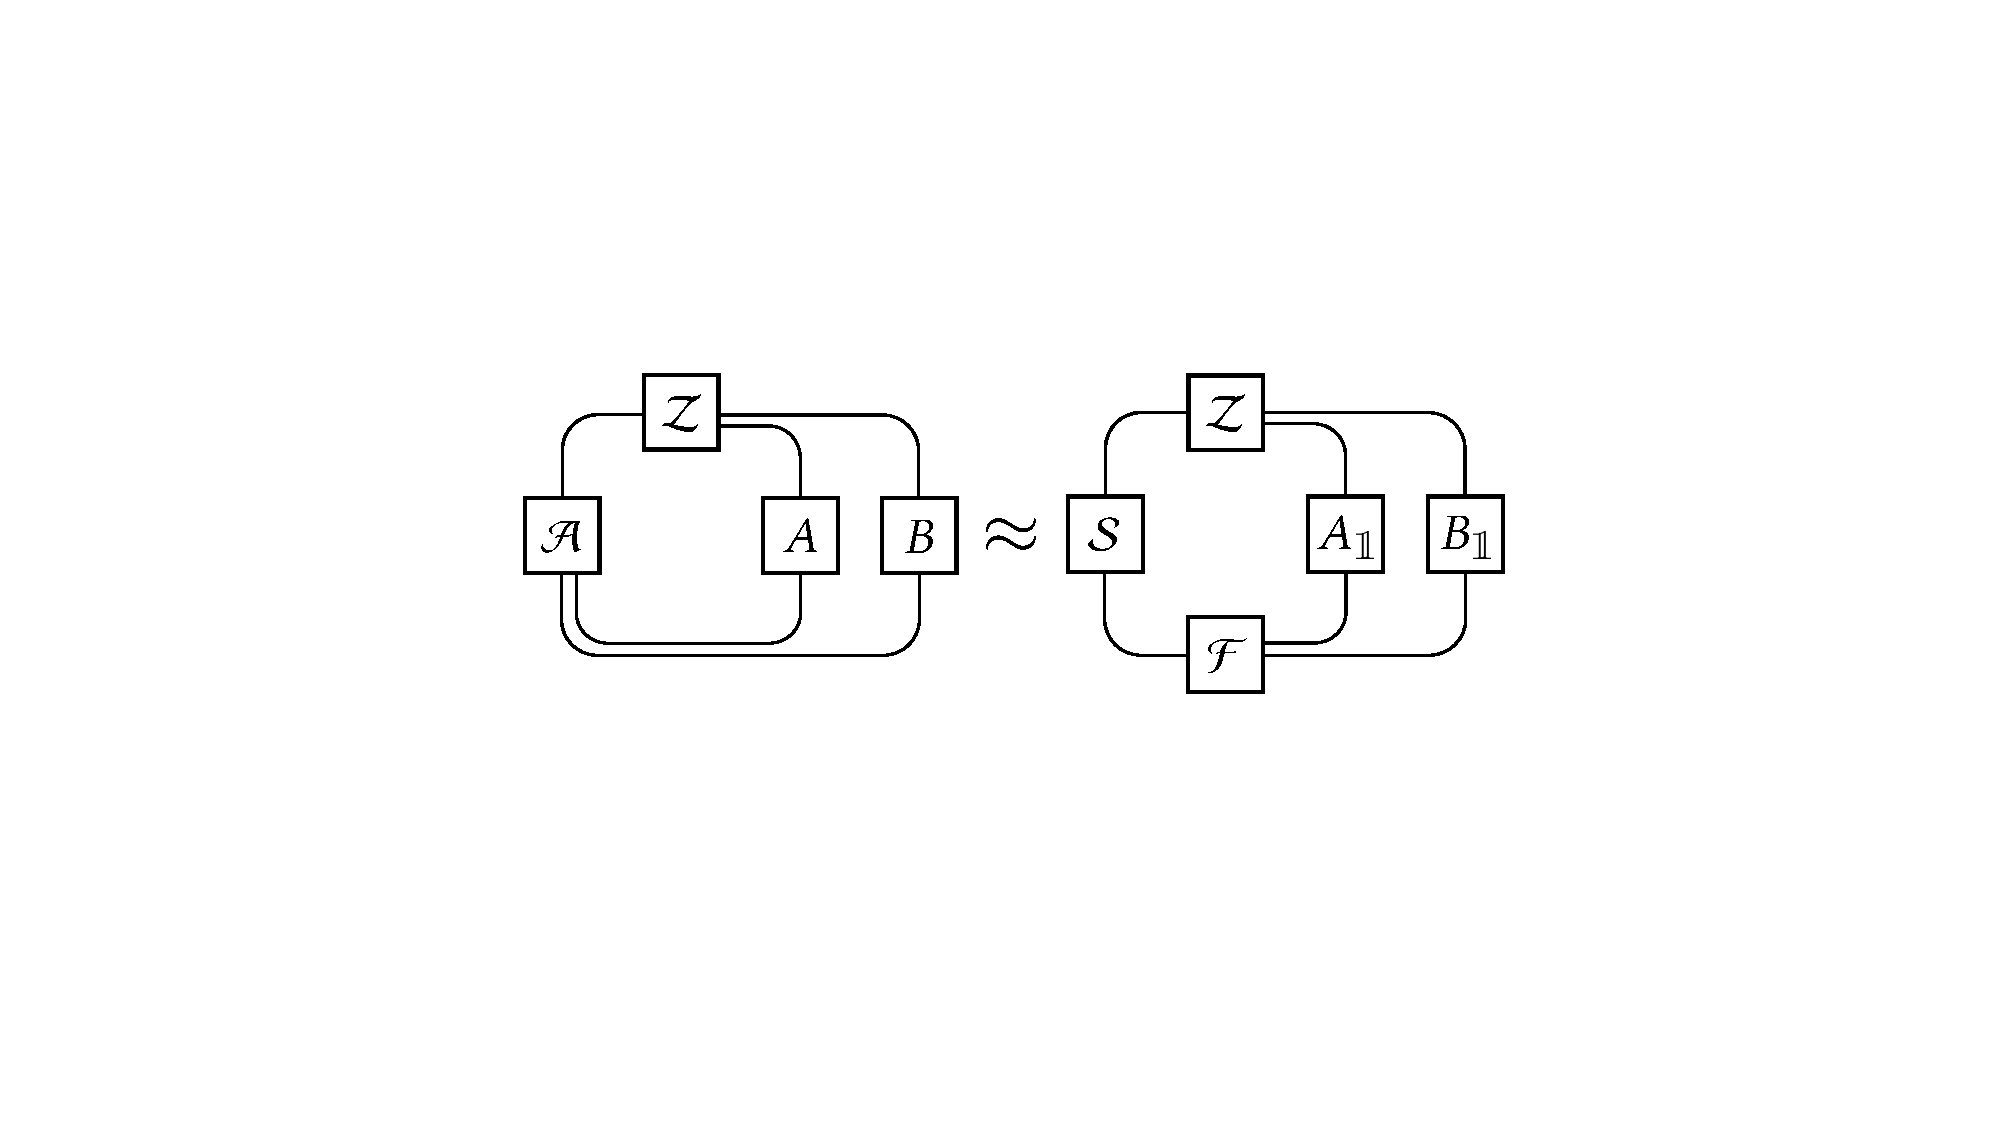
\includegraphics[width=0.85\linewidth]{graphics/suc-experiment}
  \caption{UC experiment with real world (left) and ideal world (right).}
  \label{fig:uc-experiment}
\end{figure}
All of this is indeed quite abstract, so it helps to visualize what the UC
indistinguishability experiment looks like. Figure~\ref{fig:uc-experiment}
illustrates the UC experiment with the real world on the left, the ideal world
on the right, and with communication channels as connecting lines. There are
several things worth noting here:

\begin{itemize}[leftmargin=*]
\item For simplicity, protocols have two parties: $A$ and $B$ in the real world,
  and $A_{\mathbbm{1}}$ and $B_{\mathbbm{1}}$ in the ideal world.
\item In the real world, parties $A$ and $B$ execute the protocol between
  eachother, with all messages flowing through the adversary.
\item In the ideal world, parties $A_{\mathbbm{1}}$ and $B_{\mathbbm{1}}$ are
  ``dummy'' parties, which simply relay messages between the environment
  $\mc{Z}$ and the ideal functionality $\mc{F}$.
\item An environment $\mc{Z}$ can interact with each of the worlds in the same
  way, but the main underlying difference is that it is (indirectly) interacting
  with the ideal functionality in the ideal world. If it is the case that the
  real world protocol emulates $\mc{F}$, then no environment should be able to
  tell the two worlds apart.
\end{itemize}
\end{comment}

So why bother going through all of this? The primary benefit is
\emph{modularity.}  Suppose a protocol $\pi$ emulates a functionality $\mc{F}$,
and suppose a protocol $\rho$, which uses $\mc{F}$ as a subroutine, emulates a
functionality $\mc{G}$.  Then, the protocol $\rho^{\mc{F} -> \pi}$, in which calls to
$\mc{F}$ are replaced by calls to $\pi$, also emulates $\mc{G}$!

This may seem a bit odd---the protocol $\pi$ lives in the real world and $\mc{F}$
lives in the ideal world. Indeed, we call this the \emph{$\mc{F}$-hybrid world},
and therein lies the power of UC. Instead of analyzing the composite protocol
consisting of $\rho$ and $\pi$, it suffices to analyze the security of $\rho$ by itself
in the much simpler $\mc{F}$-hybrid world, where it can make calls to
$\mc{F}$. If we can show that $\rho$ emulates $\mc{G}$ in the $\mc{F}$-hybrid
world, then we can later substitute for $\mc{F}$ any protocol that emulates it
without fear of something going wrong.

\begin{comment}
Figure~\ref{fig:uc-experiment} illustrates the UC experiment in the context of
the commitment scheme defined previously. The real world is shown on the left
and the ideal world is shown on the right, with connecting lines denoting
communication channels.\footnote{Note that in the real world, all communication
  passes through the adversary $\mc{A}$. In the bare model, communication is
  asynchronous, unauthenticated, and unreliable, but other models of
  communication can be built atop this model.} In the real world, $A$ and $B$
carry out the protocol with eachother, while in the ideal world,
$A_{\mathbbm{1}}$ and $B_{\mathbbm{1}}$ are ``dummy'' parties that simply relay
messages between $\mc{Z}$ and $\mc{F}$. The environment $\mc{Z}$ is tasked to
interact with each world and distinguish between the two.
\end{comment}

\begin{comment}
\myheader{Example: Secure coin flipping.} Suppose two untrusting parties, Alice
and Bob, wish to securely flip a coin---Alice calls the coin flip by publishing a
bit $b \in \{ 0, 1\}$, and Bob flips the coin by publishing the result $r \in \{0,
1\}$. If $b = r$, then Alice wins; otherwise, Bob wins. Observe that simply
having Alice and Bob publish their respective values is not secure. If Alice
publishes $b$ first, then Bob can cheat by manipulating $r$ in his favor (and
vice versa)!

In order to carry out the coin flip securely, they can use a commitment
scheme~\cite{brassard1988minimum}, which is the digital equivalent of a ``sealed
envelope.'' Here is the idea:
\begin{enumerate}[leftmargin=*]
\item Alice: Commit to $b$ as $C_A = \mathsf{com}(b)$, and send $C_A$ to Bob.
\item Bob: Commit to $r$ as $C_B = \mathsf{com}(r)$  and send $C_B$ to Alice.
\item Alice: Open the commitment as $b' = \mathsf{open}(C_A)$, and send it to Bob.
\item Bob: Open the commitment as $r' = \mathsf{open}(C_B)$, and send it to Bob.
\end{enumerate}
\noindent If $r' = b'$, then Alice wins; otherwise, Bob wins. But what is to stop
either party from cheating? In order for the protocol to be secure, it should
satisfy these important properties (stated informally):
\begin{itemize}[leftmargin=*]
  \item \emph{Hiding.} A commitment should not reveal any information about the
    committed value.
  \item \emph{Binding.} A commitment should only open to the originally
    committed value.
  \item \emph{Non-malleability.} One should not be able to create a commitment
    $C'$ from a commitment $C$ such that the committed values are related.
\end{itemize}

The first two properties are fairly straightforward, and indeed, they are
sufficient for security in the standalone setting and under sequential
composition. However, in the concurrent setting described here (Alice and Bob
are both running a commitment scheme), non-malleability is necessary for
security. Suppose Bob sees Alice's commitment $C_A$ first. While he cannot
figure out Alice's bit from $C_A$ (due to the hiding property), a malleable
commitment scheme might allow him to create a commitment $C_B'$ from $C_A$,
which simply flips the bit committed in $C_A$. Bob does not learn Alice's bit,
but he can still force the outcome of the game in his favor.\smallskip


\myheader{Commitment functionality.} \todo{Non-malleability is difficult to
  capture.} We can capture all of these properties at once by defining an ideal
functionality $\Func_{\textsc{com}}$ for a (one-time) commitment scheme as it
would appear in the cryptography literature (Figure~\ref{func:com}, left).

Upon receiving the bit $b$ that Alice wishes to commit to,
$\Func_{\textsc{com}}$ records $b$ and notifies Bob that it has done so. Then,
whenever Alice wants to reveal $b$ to Bob, she notifies $\Func_{\textsc{com}}$,
which sends it to Bob. Because, in this idealized world, Alice and Bob trust
$\Func_{\textsc{com}}$ to do all the work, the hiding, binding, and
non-malleability properties hold trivially. Of course, in the real world, Alice
and Bob would not want to trust such a third party (if it even exists), so their
hope is that the commitment scheme they use is ``just as good as''
$\Func_{\textsc{com}}$.
\end{comment}

\subsection{ILC By Example}
\label{subsec:ilc-flavored}

\emph{Commitment} is an essential building block in many cryptographic
protocols~\cite{brassard1988minimum}. The idea is simple: A \emph{committer}
provides a \emph{receiver} with the digital equivalent of a ``sealed envelope''
containing some value that can be later revealed. Formalizing the security
of this basic primitive, however, is nontrivial.

To obtain security in the standalone setting or under sequential composition, a
commitment should satisfy two basic properties:
\begin{itemize}[leftmargin=*]
\item \emph{Hiding.} A commitment to a value should not reveal any information
  about the value.
\item \emph{Binding.} A commitment should only open to the originally committed value.
\end{itemize}

\noindent To obtain security under concurrent composition, however, a commitment
should satisfy a third subtle property:
\begin{itemize}[leftmargin=*]
\item \emph{Non-malleability.} One should not be able to create a new commitment
  $C'$ from an unopened commitment $C$ such that the committed values are
  related in any way.
\end{itemize}

We can capture all three of these properties at once using an ideal
functionality. On the left side of Figure~\ref{func:com}, we define
$\Func_{\textsc{com}}$, an ideal functionality for one-time bit commitment, as
it would appear in the cryptography
literature~\cite{canetti2001commitments}. The functionality simply waits for the
committer $A$ to commit to some bit $b$, notifies the receiver $B$ that it has
taken place, and reveals $b$ to $B$ upon request by $A$. Notice that $B$ never
actually sees a commitment to $b$ (only the (\textsf{Receipt}) message), so the
three properties hold trivially.

On the right side of Figure~\ref{func:com}, we define $\Func_{\textsc{com}}$ in
ILC to highlight some key features of the language, such as its affine and modal
type system. Keep in mind that the overarching feature of ILC is confluence, so
many of our design choices are artifacts of reaching for this
quality. \todo{Sequential activation order?}\smallskip

\myheader{Affine types.}
%The role of affine types is to restrict the dataflow of
%read channels so that no confusion arises at the receiving ends of
%communications.
Let us first examine the function signature of \textsf{fCom}, which (glossing
over some details) takes as arguments two channels, a read channel \textsf{frA}
(reads message from $A$) and a write channel \textsf{toB} (writes messages to
$B$), and returns \textsf{Unit}. There are a number of things to unpack here:

\begin{itemize}[leftmargin=*]
  \item The signature consists of affine arrows $\multimap$ (or ``lollipops''), which
    describe the types of functions that consume their argument at most once.
  \item Both lollipops and intuitionistic (unrestricted) arrows carry the
    \emph{modal type} (or \emph{mode}) of their function bodies. A mode can have
    one of three values: either write $\Wm$, read $\Rm$, or value $\Vm$.  In the
    example, the left lollipop has mode $\Vm$, which we elide, and the right
    lollipop has mode $\Rm$. We have more to say about modes later.
  \item Channels are typed. Both \textsf{frA} and \textsf{toB} communicate
    values inhabiting the sum type \textsf{Msg}.
  \item Read channels are affinely typed to protect them from duplication.
  \item Write channels and the unit value are intuitionistically typed. Hence,
    their types require the ! operator (pronounced ``bang!'') to be lifted into
    an affine type.
\end{itemize}

\noindent ILC achieves the above with a two-kind system. That is, types are
bifurcated into a kind for intuitionistic types and a kind for affine
types.

The main takeaway of the affine type system is this: It restricts the dataflow
of read channels so that no confusion arises at the receiving ends of
communications.\smallskip

\myheader{Modal types.} ILC expressions are typed with one of three modes: $\Wm$
(write mode), $\Rm$ (read mode), or $\Vm$ (value mode). Modes can be composed
either sequentially or in parallel to yield new modes.

To give a few examples, suppose expressions $e_1$ and $e_2$ have modes $m_1$ and
$m_2$, respectively. Sequential mode composition shows up in the obvious case of
sequentially evaluating the two expressions, so the mode of the expression
$\eSeq{e_1}{e_2}$ is $m1 ;; m2 => m3$.\footnote{The expression $\eSeq{e_1}{e_2}$
  is syntactic sugar for $\eLet{\eUnit}{e_1}{e_2}$.} Parallel mode composition
shows up when one process forks a second process, so the mode of the expression
$\eFork{e_1}{e_2}$ (fork a process $e_1$ and continue as $e_2$) is $m_1 || m_2
=> m_3$. The rules for mode composition are discussed in Section~\ref{sec:ilc}.

The main takeaway of the modal type system is this: The parallel composition of
write mode processes is \emph{not allowed}, i.e., $\Wm || \Wm => p$ is not
derivable for any mode $p$. Recall that in the ITM model, execution is
essentially single-threaded, so this ensures that no confusion arises as to
which process is currently writing, or equivalently, which process is currently
active.\smallskip

\myheader{Putting it all together.} The function body of \textsf{fCom} closely
follows $\Func_{\textsc{com}}$, but there are several points worth mentioning.
First, we introduce the letrd and wr typing rules. Typing judgements have the
form $\Delta ; \Gamma |- e : A |> m$, where $\Delta$ is an affine typing context, $\Gamma$ is an
intuitionistic typing context, and $m$ is a mode.
\begin{mathpar}
\Infer{letrd}
{\Delta_1 ; \Gamma |- e_1 : \tyRd{A}\\
\Delta_2,x_1:\tyBang{A},x_2:\tyRd{A} ; \Gamma |- e_2 : B |> m
}
{\Delta_1, \Delta_2 ; \Gamma |- \eLetRd{x_1}{x_2}{e_1}{e_2} : B |> \Rm}
\end{mathpar}

The letrd rule says that if we can partition the affine context $\Delta$ as $\Delta_1,
\Delta_2$ such that $e_1$ has type $\tyRd{A}$ and mode $\Vm$ (elided) under contexts
$\Delta_1; \Gamma$, and $e_2$ has type $B$ and mode $m$ under contexts
$\Delta_2,x_1:\tyBang{A},x_2:\tyRd{A} ; \Gamma$, then the full expression has type $B$ and
mode $\Rm$. Notice several things:
\begin{itemize}[leftmargin=*]
  \item Reading on a channel of type $\tyRd{A}$ produces an affine pair (or
    ``tensor'') of type $\tyTensor{\tyBang{A}}{\tyRd{A}}$.
  \item ILC only allows intuitionistically typed values to be sent over channels
    ($A$ ranges over intuitionistic types), so the value read on the channel is
    lifted into the first element of the tensor as an affine type using the
    bang! operator.
  \item The read channel itself is rebound as the second tensor element, so that
    it may be used again.
  \item Pattern matching with the ! operator unpacks affine values, so the value
    bound to $b$ in the first read from \textsf{frA} has an intuitionistic type.
\end{itemize}
\begin{mathpar}
\Infer{wr}
{\Delta_1; \Gamma   |- e_1 : A\\
\Delta_2; \Gamma   |- e_2 : \tyWr{A}}
{\Delta_1, \Delta_2; \Gamma |- \eWr{e_1}{e_2} : \tyUnit |> \Wm}
\end{mathpar}

The wr rule says that if we can partition the affine context $\Delta$ as $\Delta_1, \Delta_2$
such that $e_1$ has type $A$ and mode $\Vm$, and $e_2$ has a type $\tyWr{A}$ and
mode $\Vm$, then the full expression has type $\tyUnit$ and mode $\Wm$.

Revisiting \textsf{fCom}, observe that the two letrd expressions are composed
sequentially, so the mode of the entire function body is derived as $\Rm ;; \Rm
=> \Rm$ according to our mode composition rules. This is reflected in the fact
that the right lollipop in the function signature carries a mode $\Rm$. Finally,
because wr expressions return $\eUnit$, we wrap it inside a bang! to lift its
type into the affine type \textsf{!Unit}.

\subsection{The UC Framework, Concretely}
\label{subsec:uc-concretely}

\todo{Preview of SaUCy and UC metatheory.}

\begin{comment}
\subsection{UC composition}
\label{subsec:composition}

The advantage of security definitions in UC is that they satisfy strong
composability guarantees, even under concurrent composition. Suppose that $\pi_1$
is a protocol that securely realizes a functionality $\mc{F}_1$. If a protocol
$\pi_2$, using $\mc{F}_1$ as a subroutine, securely realizes a functionality
$\mc{F}_2$, then the protocol $[\pi_1 / \mc{F}_1]\pi_2$, in which calls to
$\mc{F}_1$ are replaced by calls to $\pi_1$, also securely realizes
$\mc{F}_2$. That way, it suffices to analyze the security of the standalone
protocol $\pi_2$ in the $\mc{F}_1$-hybrid model, where parties run $\pi_2$ with
access to $\mc{F}_1$, as opposed to the composite protocol of $\pi_2$ and
$\pi_1$. Figure~\ref{fig:uc-composition} illustrates protocol composition. The
setup on the left represents the $\mc{F}_1$-hybrid model, and the setup on the
right represents the protocol substitution $[\pi_1 / \mc{F}_1]\pi_2$, which
maintains security.

\begin{figure}
  \centering
  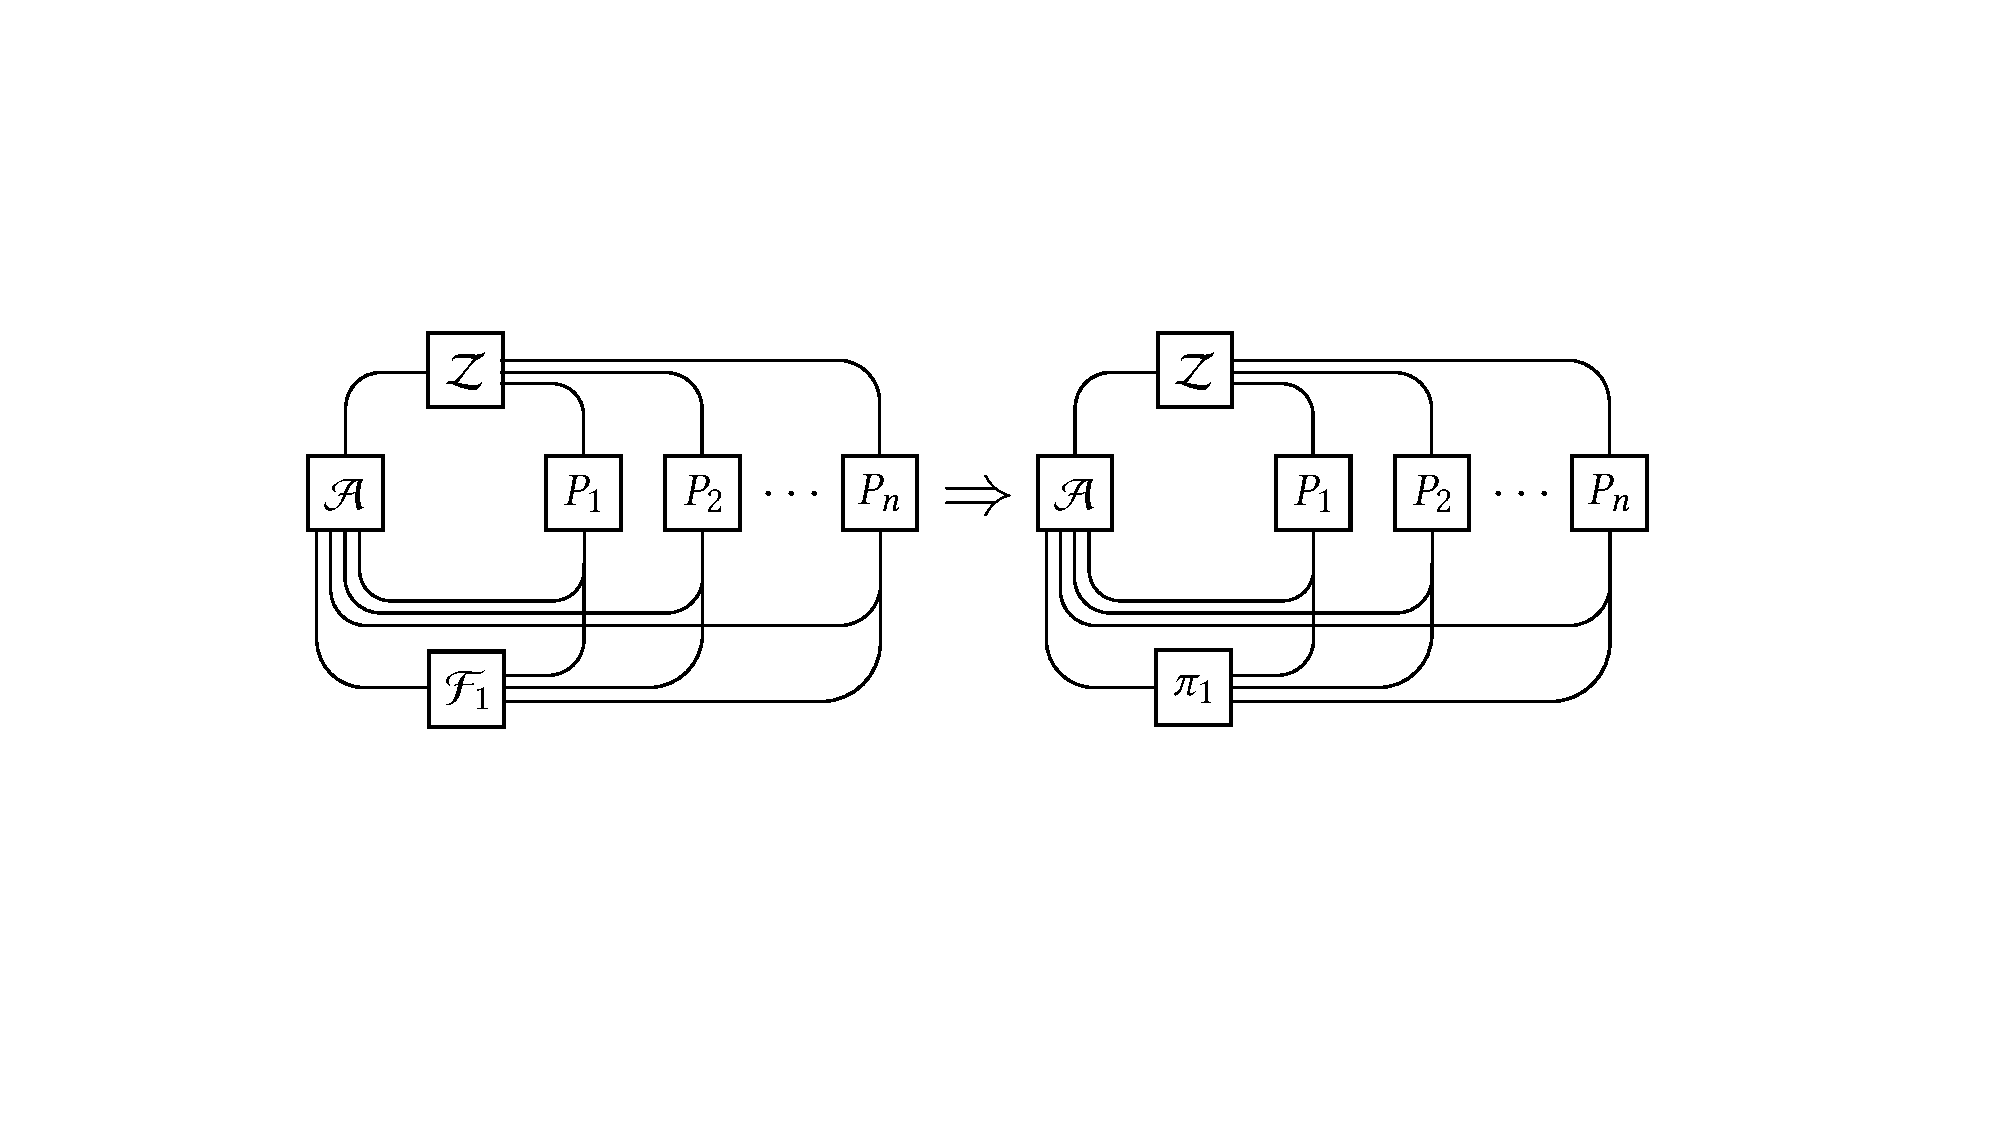
\includegraphics[width=\linewidth]{graphics/composition}
  \caption{UC protocol composition theorem.}
  \label{fig:uc-composition}
\end{figure}
\end{comment}
